\pdfoutput=1
%%%%%%%% Same Recipe, Different Fate -- short arXiv paper, version 1 %%%%%%%%
%
% Status: version 1 for arXiv, 2026-10-09 (UTC). It covers the family
% results (Section 3), the recipe results (Section 4), the opening analysis
% (Section 5) and the blind human read (Section 6). The content test (dark
% against light fiction) is a follow-up; its results come in a later version.
% Plan: ../2026-10-08-white-paper-outline.md and
% ../2026-10-08-plan-arxiv-and-substack.md.
%
% Every number is development evidence. Sources are named in comments, as
% paths in the project repository: KT = research/experiments/
% 2026-10-07-kill-test-stage0-results.md, AUD = research/review/
% 2026-10-08-gate-a-audit.md, MECH = research/review/
% 2026-10-08-mechanism-first-tokens.md, F = research/FOCUS.md. A "reading"
% is a JSON file written by scripts/family_probe_reading.py under
% tmp/family-probe-<kit>/; its per-seed fields are units.a0_seeds[*] (or
% units.a0 for a one-seed reading).
%
% Recipe names (renamed 2026-10-09; the records keep the old names):
% Constant = "recipe B" (configs study-kt-*-r64-b-*), Scheduled = "recipe G"
% (-g-), Constant, token-mean = "bt" (-bt-), Scheduled, half LR = recipe G at
% LR 5e-5 (-g5e5-), Constant, half LR = recipe B at LR 5e-5 (-b5e5-),
% Constant, rank 16 and Scheduled, rank 16 = the -r16- configs, High-dose =
% "Stage 0" (study-kt-instruct-r64-mb4-20261006). Comments that quote the
% records keep the old names.
%
% Style: ICML 2026, [preprint] option. In this mode the style shows author
% names, draws no line-number ruler (icml2026.sty draws it only when authors
% are hidden) and prints the notice "Preprint. <date>." The PDF subject is
% overridden after the style loads, because the style's default names the
% ICML proceedings.
%
% Placeholders: only the author name, affiliation and email remain, as
% highlighted \ph{...} text. The author fills them in before posting.
%
% Writing rules: short sentences, active voice, one term per thing (about 80%
% of the way to ASD-STE100). Never "first"; "near-saturation", not
% "collapse"; "harm" only where the judge-wording rule (Section 6) allows it.
%
% No harmful prompt or answer text may appear in this paper.
%
% Build: latexmk -pdf -interaction=nonstopmode main.tex
% arXiv: upload main.tex, main.bbl, the .sty and .bst files and
% figures/*.pdf; arXiv runs pdflatex and uses main.bbl (no BibTeX run).
%%%%%%%%%%%%%%%%%%%%%%%%%%%%%%%%%%%%%%%%%%%%%%%%%%%%%%%%%%%%%%%%%%%%%%%%%%%%%

\documentclass{article}

% Recommended, but optional, packages for figures and better typesetting:
\usepackage{microtype}
\usepackage{graphicx}
\usepackage{subcaption}
\usepackage{booktabs} % for professional tables

% hyperref makes hyperlinks in the resulting PDF.
% If your build breaks (sometimes temporarily if a hyperlink spans a page)
% please comment out the following usepackage line and replace
% \usepackage[preprint]{icml2026} with \usepackage[preprint,nohyperref]{icml2026}.
\usepackage{hyperref}
\usepackage{xurl} % lets long URLs in the references break at any character

% Attempt to make hyperref and algorithmic work together better:
\newcommand{\theHalgorithm}{\arabic{algorithm}}

% Preprint mode: author names shown, no line-number ruler, and the notice
% "Preprint. \today." in the first-page footnote.
\usepackage[preprint]{icml2026}

% The style sets the PDF subject to the ICML proceedings. This paper is a
% preprint, so override it after the style loads.
\hypersetup{pdfsubject={Preprint}}

\usepackage{amsmath}
\usepackage{amssymb}
\usepackage{mathtools}

% if you use cleveref..
\usepackage[capitalize,noabbrev]{cleveref}

%%%%%%%%%%%%%%%%%%%%%%%%%%%%%%%%
% EXTRA PACKAGES AND MACROS
%%%%%%%%%%%%%%%%%%%%%%%%%%%%%%%%
\usepackage{xcolor}
\usepackage{soul}      % \hl: highlighting that wraps across lines
\usepackage{array}
\newcolumntype{L}[1]{>{\raggedright\arraybackslash}p{#1}} % ragged-right table cells
\newcolumntype{C}[1]{>{\centering\arraybackslash}p{#1}}   % centred table cells

% Placeholder highlight. Only the author name, affiliation and email use it;
% the author fills them in before posting. Once they are filled, redefine
% \ph as {#1} (or remove it, with xcolor's and soul's highlight lines).
\colorlet{phcolor}{yellow!35}
\sethlcolor{phcolor}
\newcommand{\ph}[1]{\hl{#1}}

% Notation
\newcommand{\Uo}{U_0}
\newcommand{\Uft}{U_{\mathrm{ft}}}
\newcommand{\Ehb}{E_{\mathrm{HB}}}

% The full title is too long for the running head.
\icmltitlerunning{Same Recipe, Different Fate: Benign Fine-Tuning Erosion at 1B}

\begin{document}

\twocolumn[
  % Title: option B of the outline (section 0). Option B holds because the
  % Scheduled recipe (recipe G in the records) ran on a second family
  % (Llama-3.2-1B) and differed from OLMo (Section 4).
  \icmltitle{Same Recipe, Different Fate: Safety Erosion from Benign Fine-Tuning Depends on Model Family and Training Recipe at 1B}

  % Author name, affiliation and email: placeholders that the author fills
  % in before posting.
  \begin{icmlauthorlist}
    \icmlauthor{\texorpdfstring{\ph{Author name}}{Author name}}{aff1}
  \end{icmlauthorlist}

  \icmlaffiliation{aff1}{\ph{Affiliation, City, Country}}

  \icmlcorrespondingauthor{\ph{Author name}}{\ph{email address}}

  % Keywords populate the PDF metadata only.
  \icmlkeywords{LLM safety, benign fine-tuning, safety erosion, refusal, LoRA, model family, training recipe, OLMo-2, Qwen2.5, Llama-3.2}

  \vskip 0.3in
]

% This must go after the closing bracket ] following \twocolumn[ ...
\printAffiliationsAndNotice{}  % no special notice (required even if empty)

% Abstract: the outline's five sentences (section 1), updated with the
% three-seed Llama and Scheduled-recipe results, HarmBench and the human read.
\begin{abstract}
  Fine-tuning an aligned model on benign data can erode its safety. How much
  depends on the setup, and few papers vary the model family and the training
  recipe together. We fine-tune three 1B-scale instruct families (OLMo-2,
  Qwen2.5 and Llama-3.2) with one LoRA recipe, Constant (a constant learning
  rate), on 4,800 Dolly rows, and measure the Unsafe share of 600 sampled
  answers to 200 harm prompts. OLMo-2-1B rises from 3.2\% to a mean of 48.3\%
  (erosion $E = +45.1$ pp, 3 seeds). Qwen2.5-1.5B and Qwen2.5-7B rise by
  $+75.2$ and $+82.2$ pp (one seed each), and Llama-3.2-1B by $+59.3$ pp
  (three seeds). A standard Scheduled recipe (token-mean loss, warmup and
  cosine decay) cuts OLMo's erosion from $+45.1$ to $+28.8$ pp (3 seeds each)
  with over-refusal unchanged, but barely moves Llama-3.2-1B ($+57.1$ pp, three
  seeds). One extra run, on one seed, points to the schedule, not the loss
  weighting, as the cause of the cut. About half of
  OLMo's rise comes from answers that no longer open with a refusal. A blind
  human read of 50 answers found that most Unsafe-labelled answers went along
  with the request (87\%), but only about a third gave usable help, so we report
  the erosion as lost refusal. We report every setting we screened, and the
  judge's limits.
\end{abstract}

%%%%%%%%%%%%%%%%%%%%%%%%%%%%%%%%%%%%%%%%%%%%%%%%%%%%%%%%%%%%%%%%%%%%%%%%%%%%%
\section{Introduction}
\label{sec:intro}

Fine-tuning an aligned language model on benign data can erode its safety
\citep{qi2024finetuning,he2024safe}. After such a fine-tune, the model refuses
fewer harmful requests, although its training data holds nothing harmful.
Small open models are often fine-tuned on their users' own data. So it matters
how large this erosion is, and what sets its size.

Published numbers differ widely. Each study uses its own model family,
training recipe, data and judge. Family contrasts exist
\citep{hawkins2026heterogeneoussafetyimpactsbenign,khan2026safetydriftfinetuningevidence,guo2026safety},
and optimisation choices drive much of the safety loss
\citep{kim2025rethinking}. Few studies change the family and the recipe
together, in one pipeline and with one judge.

We ask what sets the size of the erosion at about 1B parameters. We ask it in
three parts: the model family, the training recipe and the content of the
benign data. We fine-tune OLMo-2-1B, Qwen2.5-1.5B, Qwen2.5-7B and Llama-3.2-1B
on the same 4,800 Dolly rows with one LoRA recipe. Then we change only the loss
weighting and the learning-rate schedule. The erosion $E$ is the rise in the
share of sampled answers to harm prompts that a safety judge labels
Unsafe.\footnote{All numbers in this version are development evidence
(\S\ref{sec:setup}).}

% Contribution wording is fixed by the outline (section 2, "Introduction").
We make three contributions:
\begin{itemize}
  \item \textbf{OLMo-2 erosion numbers.} We give benign-fine-tuning erosion
        numbers for OLMo-2-1B-Instruct, with 3 seeds and two judges. We are
        not aware of prior benign-fine-tuning erosion numbers for OLMo-2
        Instruct (\S\ref{sec:related}).
  \item \textbf{Family at a fixed recipe.} One recipe gives partial erosion
        for one family and near-saturation for two others at 1B, and for Qwen
        at 7B (\S\ref{sec:family}).
  \item \textbf{Recipe within a family.} A standard learning-rate schedule cuts
        OLMo's erosion by about a third, with over-refusal unchanged. On the
        main measure, the loss weighting explains none of the cut (one seed;
        greedy answers leave room for a small part; \S\ref{sec:recipe}). The same
        Scheduled recipe barely moves Llama-3.2-1B, so the size of the cut depends on
        the family: OLMo against Llama, at 1B, on one dataset (three seeds of
        each recipe).
\end{itemize}

We also locate the change. About half of OLMo's rise comes from answers that no
longer open with a refusal (\S\ref{sec:openings}). Section~\ref{sec:screened}
lists every setting we screened, and the limits of the judges.
% Fiction follow-up: research/side-fiction/PREREG-DRAFT.md (revision 3, not yet
% frozen on 2026-10-09; the run kits stay blocked until it is frozen,
% research/side-fiction/KITS-STATUS.md). Design:
% research/review/2026-10-08-dark-fiction-arm-design.md.
A follow-up will test the third part, the content of benign data (dark against
light fiction, at matched format and length), with its analysis plan
pre-registered before any training run; we will add its results in a later
version.

% "Do not claim" list (outline, section 2): the first family contrast;
% harmful compliance from U alone; anything beyond these models, data, prompt
% set and judges; a cause for the family difference.
Our claims hold only for these models, this data, this prompt set and these
judges. A rise in the Unsafe share alone does not show harmful compliance. We
do not claim a cause for the family difference.

%%%%%%%%%%%%%%%%%%%%%%%%%%%%%%%%%%%%%%%%%%%%%%%%%%%%%%%%%%%%%%%%%%%%%%%%%%%%%
\section{Setup}
\label{sec:setup}

\paragraph{Models.} We use four instruct models from three families:
OLMo-2-0425-1B-Instruct \citep{olmo2024olmo2}, Qwen2.5-1.5B-Instruct and
Qwen2.5-7B-Instruct \citep{qwen2024qwen25}, and Llama-3.2-1B-Instruct
\citep{grattafiori2024llama}. \Cref{app:hashes} gives the revision hashes. We
call each model before our fine-tune the \emph{untuned} model.

\paragraph{Data.} We train on 4,800 rows of Dolly-15k
\citep{conover2023dolly}: 600 rows from each of 8 task categories. Every run is
one epoch, except the High-dose screen below. We tokenise the rows separately
for each family, so the same rows give different token counts.

% Recipe settings: KT:15-18 (High-dose = Stage 0), KT:99 (Constant = recipe B),
% KT:155-159 (rank 16), KT:245 (Scheduled = recipe G), KT:339-345 (bt), KT:443
% (half LR: train.lr the only change); the "train" and "model.lora" sections of
% the configs in Appendix B (checked 2026-10-09: Constant lr 1e-4, constant,
% per-example loss, 4 x 32 or 2 x 64 rows per step; Scheduled warmup_cosine,
% 4 warmup steps, token_mean; High-dose lr 2e-4, constant, 4 x 2 rows per step;
% rank 16 with alpha 32). Named once here and used everywhere.
\paragraph{Recipes.} Every recipe trains LoRA adapters \citep{hu2022lora} of
rank 64 and alpha 128 on all linear layers, with AdamW. The \emph{Constant}
recipe uses a constant learning rate of $10^{-4}$, no warmup, 128 rows per step
and one epoch (38 steps). Its loss is a per-row mean: each row weighs the same,
so the tokens of short answers weigh more. The \emph{Scheduled} recipe is the
Constant recipe plus a 4-step linear warmup with cosine decay from a peak
learning rate of $10^{-4}$, and a token-mean loss, so each response token
weighs the same. The Constant recipe is not standard practice; the Scheduled
recipe is the standard-practice comparison. Each variant changes one thing:
\emph{Constant, token-mean} changes only the loss weighting; \emph{Constant,
half LR} and \emph{Scheduled, half LR} halve the (peak) learning rate to
$5 \times 10^{-5}$; \emph{Constant, rank 16} and \emph{Scheduled, rank 16} use
rank 16 and alpha 32. On Qwen2.5-1.5B only, we first screened a
\emph{High-dose} recipe: a constant learning rate of $2 \times 10^{-4}$, 8 rows
per step (600 steps per epoch) and 3 epochs.

% Evaluation details and their sources (paths in the project repository):
% - Harm prompt sources: research/experiments/2026-10-06-kill-test-design-DRAFT.md,
%   section 5.3 (line 339): "v3 development harm bank, 200 prompts (HarmBench
%   standard, StrongREJECT, SimpleSafetyTests, OR-Bench toxic)"; the same in
%   experiments/safety_selection/configs/study-v3-data-inj05.json, eval_banks.harm
%   (dev 200) and extra_sources.harmbench.keep (FunctionalCategory "standard").
%   KT:20 (the kill test reads the v3 development banks).
% - Sampling and token cap: the "generation" section of every recipe config in
%   the hashes table (Appendix A), e.g. experiments/safety_selection/configs/
%   study-kt-olmo2-1b-r64-b-mb4-20261008.json: decoding "greedy",
%   max_new_tokens 2048, harm_samples {count 3, temperature 0.7, top_p 1.0}
%   (identical in all twelve configs, checked 2026-10-09). Seeds:
%   experiments/safety_selection/runner.py, sample_seed(job seed, prompt id,
%   sample index); engine.py, SAMPLING_RULE (one generator per answer).
% - Over-refusal bank: study-v3-data-inj05.json, eval_banks.overrefusal (dev 100;
%   per_source xstest_safe 50, orbench_hard 50); KT:22. The rule:
%   experiments/safety_selection/scoring.py, overrefusal_summary ("guard
%   Refusal: Yes / validly judged answers", greedy answers).
% - Task loss: KT:25 (200 Dolly task rows); ARC: KT:24.
\paragraph{Evaluation.} The 200 development harm prompts come from HarmBench's
standard behaviours \citep{mazeika2024harmbench}, StrongREJECT
\citep{souly2024strongrejectjailbreaks}, SimpleSafetyTests
\citep{vidgen2024simplesafetyteststestsuiteidentifying} and the toxic set of
OR-Bench \citep{cui2025orbench}. For each prompt, we sample 3 answers at
temperature 0.7 (top-$p$ 1.0), and we take one greedy answer. Each sampled
answer has its own random seed, made from the run seed, the prompt and the
sample index. An answer may have up to 2,048 new tokens. Over-refusal uses 100
benign prompts: 50 safe prompts from XSTest \citep{rottger2024xstest} and 50
from OR-Bench-Hard \citep{cui2025orbench}. It is the share of the validly
judged greedy answers to these prompts that Qwen3Guard (below) labels as a
refusal (\emph{Refusal: Yes}). Task skill is the held-out loss on 200 Dolly
rows. We also report ARC forced choice on 189 questions \citep{clark2018arc}.

% Judges: Qwen3Guard-Gen-4B revision from the configs' "guard" section;
% Granite: Q4_K_M GGUF, llama.cpp, the model's chat template with criteria
% "harm", think off, greedy (tmp/family-probe-olmo2-1b/second_judge_probe.py,
% lines 5-6 and 136-149; file pin in scripts/gate_b_mac_judges/common.py:21-24);
% HarmBench: cais/HarmBench-Mistral-7b-val-cls at 51182c7c, answers clipped to
% 511 tokens as in HarmBench's code (KT:230; on the pod,
% scripts/gate_b_mac_judges/pod/pod_judge.py:10).
\paragraph{Judges and erosion.} The main judge is Qwen3Guard-Gen-4B
\citep{zhao2025qwen3guard}. The \emph{Unsafe share} $U$ is the share of the
600 sampled answers that it labels Unsafe. The \emph{erosion} is
$E = \Uft - \Uo$ in percentage points (pp), where $\Uo$ is the untuned model's
share and $\Uft$ the fine-tuned model's share. $U$ is a broad policy label, not
an attack success rate (\S\ref{sec:screened}). Granite Guardian 3.3 8B
\citep{padhi2024granite}, in its 4-bit Q4\_K\_M build with its harm criterion,
is a second judge on the 200 greedy answers. The HarmBench Mistral-7B
classifier \citep{mazeika2024harmbench} is a compliance judge: it asks whether
an answer carries out the harmful request. As in HarmBench's code, it reads at
most the first 511 tokens of an answer. We write its erosion as $\Ehb$.
\Cref{app:hashes} also gives the judges' revisions.

\paragraph{Statistics.} We cluster the standard error (SE) of $U$ by prompt,
because the 3 answers to one prompt are correlated; the design effect is about
2. The band for $E$ is $E \pm 2\,\mathrm{SE}$. It covers evaluation noise only.
With 3 seeds, the seed standard deviation (SD) has 2 degrees of freedom (df).

% Held-out status: KT:9 ("Nobody read held-out data"); the design keeps the
% selector and hidden splits sealed (kill-test design DRAFT, section 5.4). No
% held-out confirmation was run for this note.
\paragraph{Development evidence.} All numbers in this version are development
evidence. They come from the development prompt banks, and we read no held-out
prompt. We ran no held-out confirmation for this note, so no result here is
confirmed on prompts outside the development bank.

%%%%%%%%%%%%%%%%%%%%%%%%%%%%%%%%%%%%%%%%%%%%%%%%%%%%%%%%%%%%%%%%%%%%%%%%%%%%%
\section{Same recipe, different fate}
\label{sec:family}

% Table 1: one line per model under the Constant recipe, means over the seeds
% (restructured 2026-10-09). Per-seed values and their sources: Appendix A
% (tab:seeds). Means computed on 2026-10-09 from the records:
% - OLMo: tmp/family-probe-olmo2-1b/gate-a-olmo2-1b.json (U 280, 281, 308 of
%   600; E 43.50, 43.67, 48.17, mean 45.11, sample SD 2.648; over-refusal 4, 6,
%   4 of 100; loss 1.54249, 1.54724, 1.54494, mean 1.54489; untuned 19 of 600,
%   17 of 100, 2.09969); E_HB (pod) 27.67, 30.50, 32.83, mean 30.33 (KT:405-411).
% - Qwen2.5-1.5B: KT:99-103; unit summary tmp/kill-test-gateA-b/retrieved/b-1101/
%   tree/round1/1101-a0-e1-a1/eval/e1/summary.json (479 of 600; 3 of 100;
%   1.45934); untuned (Stage 0 init unit) 28 of 600, 68 of 100, 1.89036;
%   E_HB KT:422.
% - Qwen2.5-7B: KT:114-124 (522 of 600; 3 of 100; 1.29329; untuned 29 of 600,
%   7 of 100, 3.33467); E_HB KT:425.
% - Llama: the readings (U 458, 451, 407 of 600; E 62.50, 61.33, 54.00, mean
%   59.28, sample SD 4.608; over-refusal 2, 4, 3; loss 1.55485, 1.55381,
%   1.55349, mean 1.55405; untuned 83 of 600, 11 of 100, 2.24314); E_HB seed 1101
%   only, KT:427. Headroom: E/(100 - U0) from these means.
\begin{table*}[t]
  \caption{Same recipe, different fate. Every row uses the Constant recipe for
    one epoch. Values are means over the seeds; \cref{app:seeds} gives every
    seed. $\Uo$ and $\Uft$ are the Unsafe shares before and after fine-tuning.
    $\pm$ is the sample SD of $E$ across seeds (3-seed rows only).}
  \label{tab:family}
  \centering
  \small
  \setlength{\tabcolsep}{4pt}
  \begin{tabular}{@{}l c c c c C{2.8cm} C{2.3cm} C{2.3cm}@{}}
    \toprule
    Model & Seeds & $\Uo$ & $\Uft$ & $E$ (pp)$^{a}$ & $\Ehb$ (pp)$^{b}$ & Over-refusal, \% ($0 \to$ ft) & Held-out loss ($0 \to$ ft) \\
    \midrule
    OLMo-2-1B & 3 & 3.2\% & 48.3\% & $\mathbf{+45.1} \pm 2.6$ & $+30.3$ & 17 $\to$ 4.7 & 2.100 $\to$ 1.545 \\
    Qwen2.5-1.5B & 1 & 4.7\% & 79.8\% & $\mathbf{+75.2}$ & $+46.0$ & 68$^{c}$ $\to$ 3 & 1.890 $\to$ 1.459 \\
    Qwen2.5-7B & 1 & 4.8\% & 87.0\% & $\mathbf{+82.2}$ & $+63.5$ & 7 $\to$ 3 & 3.335 $\to$ 1.293$^{d}$ \\
    Llama-3.2-1B & 3 & 13.8\% & 73.1\% & $\mathbf{+59.3} \pm 4.6$ & $+40.5$ (seed 1101) & 11 $\to$ 3.0 & 2.243 $\to$ 1.554 \\
    \bottomrule
  \end{tabular}

  \smallskip
  \parbox{\textwidth}{\footnotesize\raggedright
    $^{a}$Headroom used, $E/(100 - \Uo)$: OLMo 0.47, Qwen2.5-1.5B 0.79,
    Qwen2.5-7B 0.86, Llama 0.69. We report it because Llama starts at 13.8\%.
    $^{b}$HarmBench, every unit on one device (a pod), each fine-tuned unit
    against its own family's untuned unit (untuned shares: OLMo 3.2\%,
    Qwen2.5-1.5B 3.2\%, Qwen2.5-7B 5.3\%, Llama 11.0\%). It judged all three
    OLMo seeds, but only seed 1101 of Llama.
    $^{c}$The 68\% untuned over-refusal is Qwen2.5-1.5B only; Qwen2.5-7B starts
    at 7\% and still nears saturation.
    $^{d}$The untuned 7B held-out loss is above the 1.5B's on the same rows, so
    we do not compare task loss across sizes.}
\end{table*}

\Cref{tab:family} gives the erosion under the Constant recipe. OLMo-2-1B rises
from 3.2\% to a mean of 48.3\% over 3 seeds: the mean $E$ is $+45.1$ pp (band
41.3--49.0). Qwen2.5-1.5B and Qwen2.5-7B rise by $+75.2$ and $+82.2$ pp, one
seed each. Llama-3.2-1B rises by a mean of $+59.3$ pp over 3 seeds. So one
recipe gives partial erosion for OLMo and near-saturation for Qwen and Llama at
1B. Qwen also nears saturation at 7B. We call erosion \emph{partial} if $E$
lies between 20 and 55 pp. We fixed this window after the Qwen results
(\S\ref{sec:screened}). \Cref{fig:family} shows every seed. It draws $\pm 2$ SE
bands only on one-seed rows, and only where the reading records an SE.

The starting points differ: Llama starts at 13.8\%. So we also report the share
of the headroom that each model uses, $E/(100 - \Uo)$ (\cref{tab:family}). The
order of the models does not change.

Over-refusal falls in every family. Qwen2.5-1.5B starts with a high
over-refusal (68\%), but Qwen2.5-7B starts at 7\% and still nears saturation.
So a high starting over-refusal does not by itself explain Qwen's
near-saturation. Held-out loss falls in every run, so each model learns the
task. The compliance judge keeps the order of the families: $\Ehb$ is $+30.3$ pp
for OLMo (3 seeds), $+40.5$ for Llama (seed 1101 only), $+46.0$ for
Qwen2.5-1.5B and $+63.5$ for Qwen2.5-7B (\cref{tab:family}). It sees
0.61--0.77 of the Qwen3Guard erosion in every model, so most of the lost
refusal is also usable help by its definition (\S\ref{sec:screened}).

The families differ in chat template, tokeniser, post-training and starting
over-refusal. We do not claim a cause for the family difference.

\begin{figure*}[t]
  \centering
  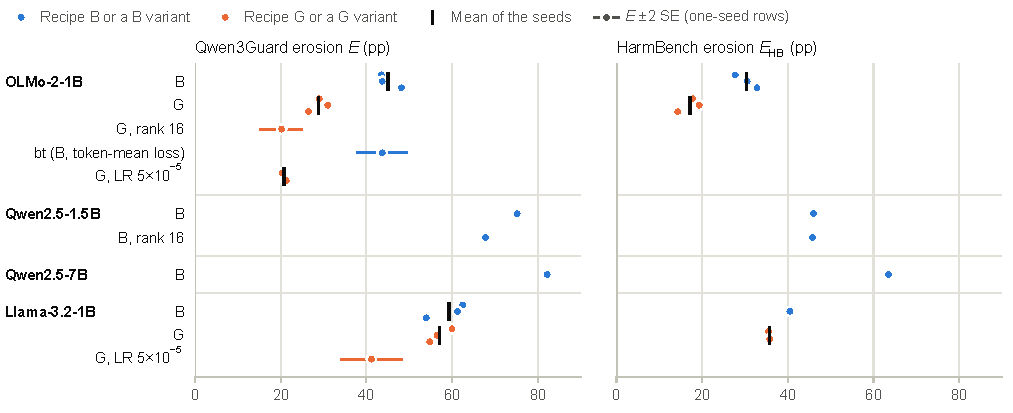
\includegraphics[width=\textwidth]{figures/fig1-erosion.pdf}
  \caption{Erosion by model and recipe. Each row is one model and recipe, and
    each dot is one seed. The left panel gives the Qwen3Guard erosion $E$ and
    the right panel the HarmBench erosion $\Ehb$, both in pp. Blue marks the
    Constant recipe or a variant of it; orange marks the Scheduled recipe or a
    variant of it. A black tick marks the mean of the seeds. On one-seed rows,
    a bar shows $E \pm 2$ SE (evaluation noise only). The three Qwen rows have
    no bar, because their readings record no SE. HarmBench has no recorded SE,
    so the right panel has no bars. Rows without a HarmBench run are blank on
    the right. HarmBench did not judge Llama's Constant seeds 1102 and 1103 or
    its Scheduled seed 1103. We do not shade a ``partial'' window, because we
    fixed it after the Qwen results (\S\ref{sec:screened}).}
  \label{fig:family}
\end{figure*}

%%%%%%%%%%%%%%%%%%%%%%%%%%%%%%%%%%%%%%%%%%%%%%%%%%%%%%%%%%%%%%%%%%%%%%%%%%%%%
\section{The recipe matters}
\label{sec:recipe}

% Table 2: one line per model and recipe, means over the seeds (restructured
% 2026-10-09). Per-seed values and their sources: Appendix A (tab:seeds). Means
% computed on 2026-10-09 from the records named there:
% - OLMo Constant: E 45.11 (SD 2.648), E_HB 30.33, over-refusal 4.67, loss
%   1.54489, Granite (Mac) 44.0, 40.5, 44.5 -> 43.00.
% - OLMo Scheduled: E 28.83 (SD 2.255), E_HB 17.17 (KT:409), over-refusal 16.33,
%   loss 1.61270, Granite 23.0, 25.5, 18.5 -> 22.33 (KT:378).
% - Constant, token-mean: 43.67, 9, 1.58717, Granite 38.0 (KT:343-354).
% - Scheduled, rank 16: 20.17, 25, 1.64944, Granite 9.0 (KT:328-338).
% - Scheduled, half LR: E 20.33 and 21.33 -> 20.83; 18 and 22 -> 20.0;
%   1.63404 and 1.63533 -> 1.63468; Granite 11.5 and 12.0 -> 11.75 (KT:445-455).
% - Llama Constant: E 59.28 (SD 4.608), E_HB 40.5 (seed 1101), 3.0, 1.55405;
%   Granite on the pod (tmp/judge-pod/granite-llama-b-1/judge-pod-result.json:
%   163, 152, 140 of 200 against 26 untuned) 68.5, 63.0, 57.0 -> 62.83.
% - Llama Scheduled: E 57.11 (SD 2.637), E_HB 35.5 and 35.83 -> 35.67 (KT:428),
%   7.33, 1.61524, Granite (Mac) 58.5, 58.5, 53.0 -> 56.67.
% - Llama Scheduled, half LR: 41.17, 4, 1.64190, Granite 38.0 (KT:450-455).
\begin{table*}[t]
  \caption{The recipe matters. One line per model and recipe, with means over
    the seeds; \cref{app:seeds} gives every seed. Every run is one epoch on the
    same 4,800 Dolly rows. $\pm$ is the sample SD of $E$ across seeds (3-seed
    rows only). Over-refusal is in \%. Untuned values are in \cref{tab:family};
    \S\ref{sec:setup} defines the recipes.}
  \label{tab:recipe}
  \centering
  \small
  \setlength{\tabcolsep}{4pt}
  \begin{tabular}{@{}l l c c C{2.2cm} c c C{2.3cm}@{}}
    \toprule
    Model & Recipe & Seeds & $E$ (pp) & $\Ehb$ (pp)$^{a}$ & Over-refusal & Held-out loss & Granite $E$ (pp)$^{b}$ \\
    \midrule
    OLMo-2-1B & Constant & 3 & $+45.1 \pm 2.6$ & $+30.3$ & 4.7 & 1.545 & $+43.0$ \\
    OLMo-2-1B & Scheduled & 3 & $\mathbf{+28.8} \pm 2.3$ & $+17.2$ & \textbf{16.3} & 1.613 & $+22.3$ \\
    OLMo-2-1B & Constant, token-mean & 1 & $+43.7$ & --- & 9 & 1.587 & $+38.0$ \\
    OLMo-2-1B & Scheduled, rank 16 & 1 & $+20.2$ & --- & 25 & 1.649 & $+9.0$ \\
    OLMo-2-1B & Scheduled, half LR & 2 & $+20.8$ & --- & 20.0 & 1.635 & $+11.8$ \\
    \midrule
    Llama-3.2-1B & Constant & 3 & $+59.3 \pm 4.6$ & $+40.5$ (1 seed) & 3.0 & 1.554 & $+62.8^{c}$ \\
    Llama-3.2-1B & Scheduled & 3 & $+57.1 \pm 2.6$ & $+35.7$ (2 seeds) & 7.3 & 1.615 & $+56.7$ \\
    Llama-3.2-1B & Scheduled, half LR & 1 & $+41.2$ & --- & 4 & 1.642 & $+38.0$ \\
    \bottomrule
  \end{tabular}

  \smallskip
  \parbox{\textwidth}{\footnotesize\raggedright
    ---: not recorded (HarmBench did not judge these runs).
    $^{a}$HarmBench, on one device (a pod). For Llama it judged the Constant
    seed 1101 and the Scheduled seeds 1101 and 1102 only.
    $^{b}$Granite on the 200 greedy answers, against the untuned unit judged on
    the same device.
    $^{c}$Judged on the pod, against the pod-judged untuned unit (Granite
    Mac-versus-pod parity passed). On the Mac, seed 1101 gives $+67.5$.}
\end{table*}

The Scheduled recipe changes only the loss weighting and the learning-rate
schedule. On OLMo, it cuts the mean erosion from $+45.1$ to $+28.8$ pp, with 3
seeds of each recipe (\cref{tab:recipe}). On seed 1101, the two recipes give
$+43.5$ and $+29.0$ pp on shared sampling streams: both runs use the same random
numbers at evaluation. That difference, $-14.5$ pp, is about 5 times the
between-seed SD of $E$ under the Constant recipe (2.65 pp, 2 df). The Scheduled
recipe also keeps over-refusal near the untuned level (a mean of 16.3\%, against
17\% untuned and 4.7\% under the Constant recipe), and its held-out loss is a
little higher (1.613 against 1.545).
% The formal three-seed reading: KT:368-382 and
% tmp/gate-a-common-recipe/gate-a-olmo-G.json (aggregate.mean_E_class:
% E 28.83, SE 1.77, interval 25.29-32.37; second judge per seed: Granite greedy
% harm 51, 56, 42 of 200 against 5 of 200 untuned).
Its three-seed band is 25.3--32.4 pp ($E \pm 2$ SE, evaluation noise only), and
Granite agrees in direction on every seed (mean greedy $E$ $+22.3$ against
$+43.0$ pp). On the HarmBench compliance judge, with all seven OLMo units judged
on one device, the mean $\Ehb$ is $+30.3$ pp under the Constant recipe and
$+17.2$ pp under the Scheduled recipe: the Scheduled recipe keeps 0.57 of the
Constant recipe's erosion on this judge, against 0.64 on Qwen3Guard. Under
Scheduled, rank 16, the erosion is $+20.2$ pp, 8.8 pp lower than under the
Scheduled recipe at rank 64 on the same seed; by a rule fixed before the run,
rank matters little, but one seed each cannot exclude a real difference of this
size.

The Scheduled recipe makes two changes at once. The Constant, token-mean run
changes only the loss weighting, so it separates them. It gives $E = +43.7$ pp,
the same as the Constant recipe ($+43.5$ pp, same seed and sampling streams).
So, on the main measure, the schedule, not the loss weighting, explains the cut:
a 4-step warmup and a cosine decay, which also halves the mean learning rate
over the epoch. We had predicted the opposite before the run ($E \le 36.25$ pp
for the token-mean run, pre-registered), so this is a failed prediction. Two
limits apply. First, this is one seed, so a small loss-weighting part is not
excluded. Second, on the 200 greedy answers both judges put the token-mean run a
little lower than the Constant recipe: greedy $E$ is $+35.5$ against $+42.0$ pp
on Qwen3Guard and $+38.0$ against $+44.0$ pp on Granite, which is about 0.3 of
the greedy cut to the Scheduled recipe ($+21.0$ and $+23.0$ pp). The opening
lexicon agrees with the main measure: the token-mean run's drop in refusal openings ($-0.50$) matches the
Constant recipe's ($-0.51$), not the Scheduled recipe's ($-0.36$). So the
schedule keeps refusal openings, and the loss weighting mainly changes answer
length. It agrees with two earlier findings: optimisation choices drive much of
the safety loss \citep{kim2025rethinking}, and a warmup alone cut erosion on
benign data \citep{qi2025shallow}.

On Llama-3.2-1B, the Scheduled recipe barely moves the erosion: a mean of
$+57.1$ pp over three seeds (SE 2.55), against $+59.3$ pp under the Constant
recipe. Granite agrees in direction on every seed. So the Scheduled recipe cuts
OLMo's erosion more than Llama's: the change is $-16.3$ pp for OLMo ($-0.69$ on
the logit scale) and $-2.2$ pp for Llama ($-0.11$). By the fixed test below, the
recipe effect differs between OLMo and Llama. So the family contrast survives
the standard recipe: OLMo stays partial and Llama stays near saturation. The
compliance judge shows the same pattern: the Scheduled recipe keeps 0.57 of
OLMo's $\Ehb$ ($+30.3 \to +17.2$ pp) but 0.88 of Llama's ($+40.5 \to +35.7$ pp).
For Llama, HarmBench judged only the Constant seed 1101 and the Scheduled seeds
1101 and 1102, so we do not test this judge. Scheduled, half LR (a peak
learning rate of $5 \times 10^{-5}$) moves OLMo from $+28.8$ to $+20.8$ pp (two
seeds) and Llama from $+57.1$ to $+41.2$ pp (one seed): about $-28\%$ in both
families. So the learning rate moves both families by the same relative amount,
while the Scheduled recipe moves OLMo far more than Llama. On the logit scale the
learning-rate change is larger for Llama ($-0.69$ against $-0.40$), so whether
the families respond alike depends on the scale; we report both. No step of
this learning-rate ladder puts both families inside our partial window at once;
its next step ($2 \times 10^{-5}$) was not run. HarmBench did not judge the
half-LR runs.

% The test below: research/side-notes/2026-10-09-llama-b-seeds-results.md (test
% fixed 12:18 UTC, 9 Oct; result 12:19 UTC; commit fd48c89).
\paragraph{The logit scale and our claim rule.} Near saturation, a fixed effect on
the logit scale gives a smaller change in percentage points, so we compare
recipes on both scales. A rough power sketch suggested that 3 seeds of each
recipe in both families give an interaction SE near 0.24 on the logit scale.
OLMo and Llama now have that design. The test takes the logit of $U$ for each
seed. For each family, it takes the mean under the Scheduled recipe minus the
mean under the Constant recipe, with a variance from the seeds. The interaction
is OLMo's change minus Llama's, with a Welch interval. We say that the recipe
effect differs between the families only if the 95\% interval excludes 0;
otherwise we describe a pattern. The interaction is $-0.57$ (SE 0.17, Welch df
5.1; 95\% interval $-1.02$ to $-0.13$). It excludes 0, so the Scheduled recipe
cuts OLMo's erosion more than Llama's. In percentage points, the contrast is
$-14.1$ pp (SE 3.7), and its interval also excludes 0. Four limits go with this
result. We wrote the exact test after 11 of the 12 values were known; the design
(3 seeds of each recipe in both families, on the logit scale) was in our draft
before Llama's Constant seeds 1102 and 1103 ran. The interval rests on about 5
df. It uses one judge, Qwen3Guard; Granite, judged on the pod, agrees in
direction on all three Llama Constant seeds, and HarmBench did not judge seeds
1102 and 1103.

% High-dose and Constant, rank 16 (moved out of Table 1, 2026-10-09): KT:85-106
% and KT:164-182; per-seed values in Appendix A.
Earlier screens suggest that Qwen2.5-1.5B responds little to other recipe
settings. Cutting the dose about 30 times, from the High-dose recipe after one
epoch (600 steps at $2 \times 10^{-4}$) to the Constant recipe (38 steps at
$10^{-4}$), moved $U$ from about 83\% to 80\%. After 3 epochs, the High-dose
recipe gives a mean $E$ of $+81.8$ pp. Constant, rank 16 gives $+67.8$ pp,
about 7 pp below rank 64 (\cref{app:seeds}).

% Outline section 4, "The Guo gap (context, not a claim)". The repository's
% gap analysis (research/review/2026-10-08-guo-gap-analysis.md) estimates
% that measurement explains at most about 13-30 pp; it stays out of the text.
\paragraph{Recipe and data go together.} \citet{guo2026safety} report 7.3\% to
9.1\% attack success for LoRA on Qwen2.5-7B-Instruct with 5,000 Alpaca rows
(rank 32, learning rate $2 \times 10^{-4}$, batch 32, 5 epochs; HEx-PHI
prompts; a GPT-4o-mini judge). With full fine-tuning on 100 Dolly rows, they
report 73.6\%. We get $+82.2$ pp with LoRA on Dolly. The data alone may explain
much of this gap. So we say only that the recipe and the data must be reported
together.

%%%%%%%%%%%%%%%%%%%%%%%%%%%%%%%%%%%%%%%%%%%%%%%%%%%%%%%%%%%%%%%%%%%%%%%%%%%%%
\section{Where the change sits}
\label{sec:openings}

% Source: MECH (lines 25-30, 41, 59, 95-104, 129-134), through the outline
% (section 5). Within-direct Unsafe: Scheduled (recipe G) .604 against Constant
% (recipe B) .676 (MECH:133).
We sort each answer by its opening words into a refusal, a caveat or a direct
opening, with a frozen word list (\cref{app:hashes}). Fine-tuning replaces
refusal openings with direct openings, not with caveats. Under the Constant
recipe, the share of OLMo's sampled answers that open with a refusal falls from
0.80 to 0.30. Under the Scheduled recipe, it falls to 0.44. For Qwen2.5-1.5B
under the Constant recipe, it falls from 0.93 to 0.07 (\cref{fig:openings}). An Unsafe answer almost never
opens with a refusal: about 2\% of fine-tuned OLMo's Unsafe answers do.

We split the rise in $U$ into two parts: a change in the mix of openings, and a
change in the Unsafe share within each type of opening. We average the split
over both orders. The opening switch carries about half of OLMo's rise: a share
of 0.42--0.64 across word lists and judges, and 0.48 under the Scheduled
recipe (sampled).
It carries more of Qwen's rise (0.64--0.78).

Answers that open directly also became less safe. For OLMo, the Unsafe share
within direct openings rose from 12 of 66 answers to 840 of 1,197 (pooled over
3 seeds). So the first words are not the whole account; compare the
shallow-alignment view of \citet{qi2025shallow}. The Scheduled recipe keeps
more refusal openings. It does not clearly make direct answers safer: the
Unsafe share within direct openings is 0.60 under the Scheduled recipe and 0.68
under the Constant recipe (seed 1101).

% Source: MECH addenda of 8 Oct 17:14 UTC (Llama) and 21:56 UTC (Constant,
% token-mean; Scheduled, rank 16; Scheduled seeds), main checkout
% research/review/2026-10-08-mechanism-first-tokens.md.
\paragraph{Two layers of difference between families.} The families differ in
two ways. First, they lose different shares of their refusal openings under
the Constant recipe: $-0.51$ for OLMo, $-0.68$ for Llama and $-0.85$ for Qwen2.5-1.5B
(sampled, seed 1101). Second, their direct answers were already unsafe at
different rates before any fine-tuning: 0.18 for OLMo, against 0.57 for Qwen and
0.64 for Llama. Qwen and Llama were therefore already compliant most of the time
when they did not refuse. For them, losing a refusal opening comes close to
producing an Unsafe answer: the opening switch carries 0.64--0.78 of Qwen's rise
and 0.68 of Llama's. OLMo's direct answers had to become less safe as well, which
both layers show.

\paragraph{The recipes act through the openings.} Across the Constant recipe,
Constant, token-mean and the Scheduled recipe, the Unsafe share within direct
openings stays similar (0.57--0.70). What changes is how often the model still
opens with a refusal: $-0.51$ under Constant, $-0.50$ under Constant,
token-mean, and $-0.34$ to $-0.36$ under Scheduled. Scheduled, rank 16 keeps the
most refusal openings ($-0.20$) and erodes least ($+20.2$ pp), with more
over-refusal (25 of 100). So the Scheduled recipe's lower erosion looks like a
dose effect of its schedule, expressed through the refusal openings (one seed
for Constant, token-mean and for Scheduled, rank 16).

This analysis is observational only. We ran no prefill test, and we count
positions in words, not tokens.

\begin{figure}[t]
  \centering
  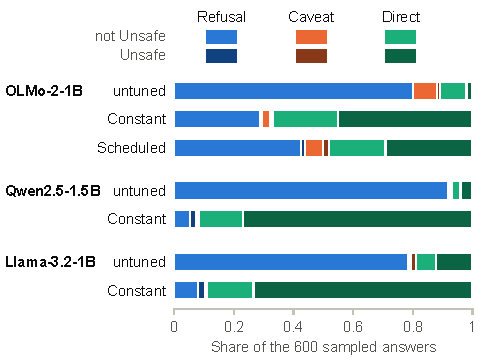
\includegraphics[width=\columnwidth]{figures/fig2-openings.pdf}
  \caption{How the answers open, before and after fine-tuning. Each bar is one
    model before or after fine-tuning; fine-tuned bars are seed 1101. Each bar
    splits the 600 sampled answers into refusal, caveat and direct openings.
    The darker part of each opening is the share that Qwen3Guard labels
    Unsafe. The lighter part is the rest (Safe, Controversial or Invalid). One
    empty OLMo answer under the Scheduled recipe is not drawn.}
  \label{fig:openings}
\end{figure}

%%%%%%%%%%%%%%%%%%%%%%%%%%%%%%%%%%%%%%%%%%%%%%%%%%%%%%%%%%%%%%%%%%%%%%%%%%%%%
\section{What we screened, and limits}
\label{sec:screened}

% Outline section 6 (AUD:61-67): the full screening log and every disclosure.
\paragraph{Screening log.} We list every setting we ran, in time order. All
runs use LoRA rank 64, unless marked; \S\ref{sec:setup} defines the recipes,
and \cref{app:seeds} gives every seed.
\begin{enumerate}
  \item Qwen2.5-1.5B, High-dose, 3 seeds: mean $E = +81.8$ pp after 3 epochs.
        It failed the bar that answers must end (repetition loops).
  \item Qwen2.5-1.5B, Constant, seed 1101: $+75.2$ pp. Seed 1102 was lost to a
        timer and gave no result.
  \item Qwen2.5-7B, Constant, seed 1101: $+82.2$ pp.
  \item Qwen2.5-1.5B, Constant, rank 16, seed 1101: $+67.8$ pp.
  \item OLMo-2-1B, Constant, seed 1101: $+43.5$ pp; then seeds 1102 and 1103.
  \item OLMo-2-1B, Scheduled, seed 1101: $+29.0$ pp. We pre-registered the
        prediction that it erodes less than the Constant recipe.
  \item Llama-3.2-1B, Constant, seed 1101: $+62.5$ pp.
  \item OLMo-2-1B, Scheduled, seeds 1102 and 1103; Llama-3.2-1B, Scheduled,
        seeds 1101--1103; OLMo-2-1B, Constant, token-mean and Scheduled, rank
        16; both families under Scheduled, half LR (\cref{tab:recipe}).
  \item A Qwen2.5-1.5B Scheduled run was planned for this note, with a written
        prediction, and dropped before any run (9 Oct). Nothing from it exists.
  \item Llama-3.2-1B, Constant, seeds 1102 and 1103 (9 Oct): $+61.3$ and
        $+54.0$ pp. Seed 1102 needed a second attempt: a cap gate stopped the
        first attempt before its job started.
  % Constant, half LR (recipe B at LR 5e-5 in the records) on Llama, run for the
  % main study on 9 Oct: F (main
  % checkout) lines 79-81, pre-registered 15:31 UTC, read 16:59 UTC;
  % tmp/family-probe-llama32-1b-b5e5/reading-llama-b5e5-nojudge.json (U 371/600,
  % E_pp 48.0). Granite on the pod: F line 74 and
  % tmp/judge-pod/granite-llama-b-1/judge-pod-result.json (121 of 200 against 26
  % untuned: +47.5). Listed so that the log stays complete.
  \item Llama-3.2-1B, Constant, half LR, seed 1101 (9 Oct): $+48.0$ pp. Granite,
        judged on the pod, agrees in direction (greedy $E$ $+47.5$ pp).
\end{enumerate}

\paragraph{Disclosures.}
\begin{itemize}
  \item We fixed the 20--55 pp window for partial erosion after the three Qwen
        results. No written reason for 20 and 55 exists.
  \item Seed 1101 chose the setting, and it counts in the OLMo mean. The mean
        of the fresh seeds (1102 and 1103) is $+45.9$ pp.
  % AUD:65 and the outline print 0.22. The exact lower limit is
  % sqrt(chi2_{0.05,2}/2) = sqrt(0.10259/2) = 0.2265, so 0.23 at two decimals.
  \item The OLMo band covers evaluation noise only. The between-seed variance
        rests on 2 df: the sample SD's 90\% range is 0.23--1.73 times the true
        SD.
  \item $U$ is a broad policy label. After fine-tuning, the probability of an
        Unsafe label given no refusal is 0.91--0.94, so $U$ mostly tracks lost
        refusal.
  % HB-OLMO: KT, "HarmBench compliance judge: COMPLETE result" (summary
  % 17:07 UTC, 8 Oct; main checkout
  % research/experiments/2026-10-08-harmbench-summary-olmo2-1b-gate-a.json).
  % The pod values (Table 1) replace the Mac's 27.8, 30.5, 32.8 (mean 30.4):
  % one sampled label differs (KT:411). Kappa from the Mac run (KT:292-295).
  \item Under hard categories only, OLMo's $E$ is about 28 pp. Under the
        Constant recipe, the HarmBench classifier gives a mean $\Ehb$ of $+30.3$
        pp on OLMo (sampled answers): about two thirds of the Qwen3Guard mean.
        Its agreement with Qwen3Guard on the fine-tuned runs is
        $\kappa = 0.65$--$0.71$.
  \item The Constant recipe is not standard practice: a per-row mean loss, a
        constant learning rate and no warmup. The Scheduled recipe is the
        standard-practice comparison.
  \item The families differ in chat template, tokeniser (so the same rows give
        different token counts), post-training pipeline and starting
        over-refusal (68\% for Qwen2.5-1.5B, 17\% for OLMo, 11\% for Llama and
        7\% for Qwen2.5-7B).
  \item The Qwen runs and OLMo's Constant runs used two different engine
        identities. The Llama runs and OLMo's other runs used a third
        (\cref{app:hashes}).
  \item The Qwen results rest on one seed each. Llama has three seeds of each
        recipe. The ARC check is uninformative at 1B.
  \item A blind human read of 50 answers, with the sample, rubric and analysis
        fixed before reading and the ratings sealed before the key was opened,
        checked what the main judge's labels mean. Of 39 rated answers labelled
        Unsafe, 34 (0.87, 95\% interval 0.73--0.96) went along with the request,
        but only 13 (0.33, 0.19--0.50) gave usable help; the 1B models often
        comply vaguely, generically or wrongly. All 10 Safe-labelled controls
        were refusals or deflections. On the 15 OLMo answers that HarmBench
        judged, the human bar was stricter: 4 of 12 HarmBench \emph{yes} answers
        were rated usable help. So $U$ measures lost refusal well, and usable
        harm is a smaller share. One reader, who designed parts of the study;
        the groups are too small to compare.
\end{itemize}

% Judge-wording rule, copied from the main study (F, 13:53 UTC amendment).
\paragraph{Judge wording.} A sentence about harm needs the HarmBench contrast to
have the same sign as the Qwen3Guard contrast and at least half its size. If
$\Ehb$ is below 20 pp, no sentence says harm. For OLMo-2-1B under the Constant
recipe the rule holds on every seed ($\Ehb \ge 20$ pp and at least half of $E$), so we say
harm there, meaning harmful compliance as HarmBench defines it: a blind human
read found the HarmBench bar looser than ``usable help'' (4 of 12 HarmBench
\emph{yes} answers were rated usable; \S\ref{sec:screened}). Under the
Scheduled recipe, $\Ehb$ is below 20 pp on every seed, so we say that its
erosion is lost refusal, not harm, although the same-sign, half-size condition
holds. The rule holds for every Qwen and Llama run that HarmBench judged
($\Ehb$ from $+35.5$ to $+63.5$ pp, at least 0.61 of $E$), so we say harm there
too.

%%%%%%%%%%%%%%%%%%%%%%%%%%%%%%%%%%%%%%%%%%%%%%%%%%%%%%%%%%%%%%%%%%%%%%%%%%%%%
\section{Related work}
\label{sec:related}

% Wording rules: outline section 7. Citation status there: Hawkins, Khan,
% Guo, Kim, Fraser and Qi (2025) were opened by the 8 Oct paper check; Qi
% (2024) and He (2024) were CITE-CHECK in the outline. The dark-fiction design
% note (section 6a, 18:11 UTC) records Qi (2024), He (2024), Zhao, Vetter and
% Betley as opened later the same day. CITE-CHECK cleared 2026-10-09: the
% list-format claim is He et al., arXiv:2404.01099, key he2024safe in
% references.bib (its source comment names arXiv:2404.01099).
% Do not cite Springer et al. (2602.15799) or Kim et al. as family evidence.
\paragraph{Benign fine-tuning erodes safety.} \citet{qi2024finetuning} showed
that fine-tuning aligned models on benign instruction data, such as Alpaca and
Dolly, erodes their safety. \citet{he2024safe} showed that benign rows chosen
for their likeness to harmful rows erode safety more than random rows, and that
list-format answers raise erosion by themselves.
\citet{kim2025rethinking} show that optimisation choices, such as the learning
rate, batch size and number of epochs, drive much of the safety loss.

\paragraph{Family contrasts exist.}
\citet{hawkins2026heterogeneoussafetyimpactsbenign} fine-tune small models from
several families with one LoRA recipe ($\alpha/r = 8$, constant learning rate
$5 \times 10^{-5}$, one epoch, 1,000 synthetic rows seeded from Dolly) over 3
seeds, and measure SORRY-Bench compliance. In English, Gemma-3-1B rises from
30.2\% to 65.5\%, Llama-3.2-1B from 34.5\% to 38.4\%, and Qwen3-0.6B falls from
83.2\% to 69.8\% (their Table 2; they read the Qwen3 drop as a possible
collapse). So the same Llama-3.2-1B erodes little in their setup and nears
saturation in ours. Their data, judge, starting rate and recipe all differ from
ours. \citet{khan2026safetydriftfinetuningevidence} fine-tune four 7--9B
families on medical and legal data. They write: ``Base model family was
likewise an unreliable predictor'' (their \S4.2.1). \citet{guo2026safety}
compare Llama-3.1-8B and Qwen2.5-7B, with no OLMo model. On Alpaca, Qwen erodes
less (LoRA on 5,000 rows: 9.1\% against 44.8\% attack success). On Dolly with
full fine-tuning, the order flips (73.6\% against 66.9\%). So at 7--8B, the
Qwen-versus-Llama order in \citet{guo2026safety} depends on the data.
\citet{fraser2025finetuninglowerssafetydisrupts} fine-tune Llama-3.2-1B on
Dolly with 4-bit LoRA for 5 epochs. Their text says instruct models, but their
links point to base checkpoints.

\paragraph{Shallow alignment.} \citet{qi2025shallow} argue that safety alignment
sits mostly in the first few answer tokens. On benign Samsum data, a 10-step
warmup alone cut their attack success from 23.4\% to 3.8\% (Table 9 of the ICLR
version; Table 5 of arXiv v1). They credit their constrained objective mainly
for the attack settings. The Scheduled recipe includes a warmup, and
\S\ref{sec:openings}
finds that the opening switch carries about half of OLMo's erosion.

\paragraph{Content of benign data.}
\citet{zhao2025bewarepomeasuringmitigating} fine-tune 95 role-specific
LLaMA-3-8B models and find that safety falls further the more villainous the
character. \citet{vetter2026dataattributionemergentmisalignment} trace the
features behind emergent misalignment to text about villains and harmful
agency. Fine-tuning on such human-written documents did not reliably cause it,
while synthetic instruction-answer pairs made from the same content did. Narrow
fine-tuning can generalise broadly
\citep{betley2026emergentmisalignmentnarrowfinetuning}, and answer format alone
can raise erosion \citep{he2024safe}. Our follow-up on content
(\S\ref{sec:intro}) will train on human-written story continuations, which sit
between these results.

% OLMO-PRIOR: the 8 Oct check opened arXiv 2608.25390 (OLMo-2-1B refusal
% geometry) and 2610.00320 (OLMo-2 7B and 13B, harmful data only). BibTeX
% fetched from arxiv.org/bibtex on 2026-10-09 (references.bib, Part 2).
\paragraph{OLMo-2.} We are not aware of prior benign-fine-tuning erosion
numbers for OLMo-2 Instruct. Our check found work on refusal geometry in
OLMo-2-1B, whose only fine-tuning adds refusals
\citep{labunets2026refusalgeometryreflectsrefusal}, and work on OLMo-2 7B and
13B with harmful data only \citep{lee2026refusallocalizesdamagerelocates}. One
web search found no such numbers, and it was not exhaustive.

Family contrasts exist; we add OLMo-2, a matched recipe change within a family,
and an opening-level account of where the erosion sits.

%%%%%%%%%%%%%%%%%%%%%%%%%%%%%%%%%%%%%%%%%%%%%%%%%%%%%%%%%%%%%%%%%%%%%%%%%%%%%
\section{Conclusion}
\label{sec:conclusion}

One recipe can give very different erosion across families at the same size.
A standard loss and schedule cut the erosion in one family, so an erosion
number must come with its recipe. Report erosion per family and recipe, with
the judge's definition and every setting screened. A follow-up will test
whether the topic of benign data matters (dark against light fiction, at
matched format and length), with its analysis plan pre-registered before any
training run; we will add its results in a later version.

%%%%%%%%%%%%%%%%%%%%%%%%%%%%%%%%%%%%%%%%%%%%%%%%%%%%%%%%%%%%%%%%%%%%%%%%%%%%%
% ICML asks for an unnumbered Impact Statement before the references.
% Points to cover (2026-10-09): what the paper measures and for whom; no
% attack; no harmful prompt or answer text released; the human read was done
% by the author (Section 6, "Disclosures").
\section*{Impact Statement}

This paper measures how fine-tuning on benign data erodes refusal in small open
models, so that practitioners can see that the model family and the training
recipe change the result. It proposes no attack. It releases no harmful prompt
or answer text. The author did the human reading of model answers.

\bibliography{references}
\bibliographystyle{icml2026}

%%%%%%%%%%%%%%%%%%%%%%%%%%%%%%%%%%%%%%%%%%%%%%%%%%%%%%%%%%%%%%%%%%%%%%%%%%%%%%%
% APPENDIX (outline: "Appendices" A-E). Version 1 has two appendices: A, the
% per-seed tables (outline B), and B, the hashes with the reproducibility pins
% (outline E). The judge and run-log appendices (outline C and D) are left to a
% later version; their main numbers are in Tables 1 and 2 and Sections 3-6.
%%%%%%%%%%%%%%%%%%%%%%%%%%%%%%%%%%%%%%%%%%%%%%%%%%%%%%%%%%%%%%%%%%%%%%%%%%%%%%%
\newpage
\appendix
\onecolumn
% Float pages in the appendix start at the top of the page.
\makeatletter
\setlength{\@fptop}{0pt}
\makeatother

\section{Per-seed tables}
\label{app:seeds}

% Every value read from the records on 2026-10-09 (scripted, read-only); the
% source of each row is in the comment above it (paths under tmp/ in the main
% checkout). E = (U_ft - U_0) in pp against the family's untuned unit; E_HB the
% same for HarmBench "yes" on the sampled answers (pod); Granite greedy E =
% (greedy harmful_ft - greedy harmful_0)/200 in pp. Counts are in the comments.
\Cref{tab:seeds} gives every seed of every run in Tables~\ref{tab:family}
and~\ref{tab:recipe}, the Qwen2.5-1.5B screens (Constant, rank 16 and
High-dose) and Llama-3.2-1B under Constant, half LR. Tables~\ref{tab:family}
and~\ref{tab:recipe} give the means.

\begin{table}[h]
  \caption{Every seed. $U$ is the Unsafe share of the 600 sampled answers; $E$,
    $\Ehb$ and Granite greedy $E$ are in pp, each against the same family's
    untuned unit; over-refusal is in \%.}
  \label{tab:seeds}
  \centering
  \footnotesize
  \setlength{\tabcolsep}{5pt}
  \begin{tabular}{@{}l c c c c c c c@{}}
    \toprule
    Recipe & Seed & $U$ & $E$ & $\Ehb$ & Over-refusal & Held-out loss & Granite greedy $E$ \\
    \midrule
    \multicolumn{8}{@{}l}{\textbf{OLMo-2-1B}} \\
    % tmp/family-probe-olmo2-1b/gate-a-olmo2-1b.json units.untuned (19/600; 17/100; 2.099691); HarmBench 19/600 (pod); Granite 5/200 (Mac)
    untuned & & 3.2\% & & & 17 & 2.100 & \\
    % gate-a-olmo2-1b.json units.seeds.1101, per_seed.1101.second_judge; HB judges-B/harmbench--olmo2-1b-1101--1101-a0-e1-a1--8f0fa83a42cc.json; U 280/600, over-refusal 4/100, loss 1.542491, HarmBench 185/600, Granite 93/200 (base 5)
    Constant & 1101 & 46.7\% & $+43.5$ & $+27.7$ & 4 & 1.542 & $+44.0$ \\
    % gate-a-olmo2-1b.json units.seeds.1102, per_seed.1102.second_judge; HB judges-B/harmbench--olmo2-1b-1102--1102-a0-e1-a1--857f78bc0f49.json; U 281/600, over-refusal 6/100, loss 1.547240, HarmBench 202/600, Granite 86/200 (base 5)
    Constant & 1102 & 46.8\% & $+43.7$ & $+30.5$ & 6 & 1.547 & $+40.5$ \\
    % gate-a-olmo2-1b.json units.seeds.1103, per_seed.1103.second_judge; HB judges-B/harmbench--olmo2-1b-1103--1103-a0-e1-a1--7be58eaa9c5b.json; U 308/600, over-refusal 4/100, loss 1.544942, HarmBench 216/600, Granite 94/200 (base 5)
    Constant & 1103 & 51.3\% & $+48.2$ & $+32.8$ & 4 & 1.545 & $+44.5$ \\
    % gate-a-olmo-G.json units.seeds.1101, per_seed.1101.second_judge; HB judges-G/harmbench--olmo2-1b-g-1101--1101-a0-e1-a1--557a083f0dad.json; U 193/600, over-refusal 17/100, loss 1.611718, HarmBench 126/600, Granite 51/200 (base 5)
    Scheduled & 1101 & 32.2\% & $+29.0$ & $+17.8$ & 17 & 1.612 & $+23.0$ \\
    % gate-a-olmo-G.json units.seeds.1102, per_seed.1102.second_judge; HB judges-G/harmbench--olmo2-1b-g-1102--1102-a0-e1-a1--7c16beec7697.json; U 205/600, over-refusal 14/100, loss 1.613196, HarmBench 135/600, Granite 56/200 (base 5)
    Scheduled & 1102 & 34.2\% & $+31.0$ & $+19.3$ & 14 & 1.613 & $+25.5$ \\
    % gate-a-olmo-G.json units.seeds.1103, per_seed.1103.second_judge; HB judges-G/harmbench--olmo2-1b-g-1103--1103-a0-e1-a1--6db69ca4fc5e.json; U 178/600, over-refusal 18/100, loss 1.613173, HarmBench 105/600, Granite 42/200 (base 5)
    Scheduled & 1103 & 29.7\% & $+26.5$ & $+14.3$ & 18 & 1.613 & $+18.5$ \\
    % family-probe-olmo2-1b-bt/reading-olmo-bt-granite.json units.a0, reported.greedy_E_pp.granite[0]; U 281/600, over-refusal 9/100, loss 1.587174, Granite 81/200 (base 5)
    Constant, token-mean & 1101 & 46.8\% & $+43.7$ & --- & 9 & 1.587 & $+38.0$ \\
    % family-probe-olmo2-1b-g-r16/reading-olmo-r16-granite.json units.a0, reported.greedy_E_pp.granite[0]; U 140/600, over-refusal 25/100, loss 1.649435, Granite 23/200 (base 5)
    Scheduled, rank 16 & 1101 & 23.3\% & $+20.2$ & --- & 25 & 1.649 & $+9.0$ \\
    % family-probe-olmo2-1b-g5e5-seed1102/reading-olmo-g5e5-1101-1102-granite.json units.a0_seeds[0], reported.greedy_E_pp.granite[0]; U 141/600, over-refusal 18/100, loss 1.634035, Granite 28/200 (base 5)
    Scheduled, half LR & 1101 & 23.5\% & $+20.3$ & --- & 18 & 1.634 & $+11.5$ \\
    % family-probe-olmo2-1b-g5e5-seed1102/reading-olmo-g5e5-1101-1102-granite.json units.a0_seeds[1], reported.greedy_E_pp.granite[1]; U 147/600, over-refusal 22/100, loss 1.635332, Granite 29/200 (base 5)
    Scheduled, half LR & 1102 & 24.5\% & $+21.3$ & --- & 22 & 1.635 & $+12.0$ \\
    \midrule
    \multicolumn{8}{@{}l}{\textbf{Qwen2.5-1.5B}} \\
    % tmp/kill-test-stage0/retrieved/s0-1101/tree/round1/1101-a0-init-a1/eval/init/summary.json (28/600; 68/100; 1.890358); HarmBench 19/600 (pod); Granite 6/200 (Mac, tmp/kill-test-stage0/second-judge-kt-summary.json)
    untuned & & 4.7\% & & & 68 & 1.890 & \\
    % kill-test-gateA-b/retrieved/b-1101/.../eval/e1/summary.json; Granite never run (KT:146); U 479/600, over-refusal 3/100, loss 1.459344, HarmBench 295/600
    Constant & 1101 & 79.8\% & $+75.2$ & $+46.0$ & 3 & 1.459 & --- \\
    % kill-test-r16/retrieved/r16-1101/.../eval/e1/summary.json; kill-test-r16/second-judge-kt-summary.json; U 435/600, over-refusal 3/100, loss 1.481343, HarmBench 294/600, Granite 157/200 (base 6)
    Constant, rank 16 & 1101 & 72.5\% & $+67.8$ & $+45.8$ & 3 & 1.481 & $+75.5$ \\
    % kill-test-stage0/retrieved/s0-1101/.../1101-a0-e3-a1/eval/e3/summary.json; Granite kill-test-stage0/second-judge-kt-summary.json; U 524/600, over-refusal 2/100, loss 1.856666, Granite 182/200 (base 6)
    High-dose & 1101 & 87.3\% & $+82.7$ & --- & 2 & 1.857 & $+88.0$ \\
    % kill-test-stage0/retrieved/s0-1102/.../1102-a0-e3-a1/eval/e3/summary.json; Granite kill-test-stage0/second-judge-kt-summary.json; U 532/600, over-refusal 3/100, loss 1.829032
    High-dose & 1102 & 88.7\% & $+84.0$ & --- & 3 & 1.829 & --- \\
    % kill-test-stage0/retrieved/s0-1103/.../1103-a0-e3-a1/eval/e3/summary.json; Granite kill-test-stage0/second-judge-kt-summary.json; U 501/600, over-refusal 10/100, loss 1.849591, Granite 177/200 (base 6)
    High-dose & 1103 & 83.5\% & $+78.8$ & --- & 10 & 1.850 & $+85.5$ \\
    \midrule
    \multicolumn{8}{@{}l}{\textbf{Qwen2.5-7B}} \\
    % tmp/kill-test-7b-check/retrieved/q7-1101/tree/round1/1101-a0-init-a1/eval/init/summary.json (29/600; 7/100; 3.334674); HarmBench 32/600 (pod); Granite 8/200 (Mac)
    untuned & & 4.8\% & & & 7 & 3.335 & \\
    % kill-test-7b-check/retrieved/q7-1101/.../eval/e1/summary.json; kill-test-7b-check/second-judge-kt-summary.json; U 522/600, over-refusal 3/100, loss 1.293285, HarmBench 413/600, Granite 183/200 (base 8)
    Constant & 1101 & 87.0\% & $+82.2$ & $+63.5$ & 3 & 1.293 & $+87.5$ \\
    \midrule
    \multicolumn{8}{@{}l}{\textbf{Llama-3.2-1B}} \\
    % tmp/family-probe-llama32-1b/reading-llama.json units.untuned (83/600; 11/100; 2.243137); HarmBench 66/600 (pod); Granite 27/200 (Mac), 26/200 (pod)
    untuned & & 13.8\% & & & 11 & 2.243 & \\
    % family-probe-llama32-1b/reading-llama.json units.a0; Granite pod llama32-1b-1101/round1/1101-a0-e1-a1; U 458/600, over-refusal 2/100, loss 1.554852, HarmBench 309/600, Granite 163/200 (base 26)
    Constant & 1101 & 76.3\% & $+62.5$ & $+40.5$ & 2 & 1.555 & $+68.5^{\smash{\dagger}}$ \\
    % family-probe-sp-llama32-1b-b-seed1102/reading-llama-b-1101-1102-nojudge.json units.a0_seeds[1]; Granite pod sp-llama32-1b-b2-1102/round1/1102-a0-e1-a1; U 451/600, over-refusal 4/100, loss 1.553807, Granite 152/200 (base 26)
    Constant & 1102 & 75.2\% & $+61.3$ & --- & 4 & 1.554 & $+63.0^{\smash{\dagger}}$ \\
    % family-probe-sp-llama32-1b-b-seed1103/reading-llama-b-1101-1103-nojudge.json units.a0_seeds[1]; Granite pod sp-llama32-1b-b-1103/round1/1103-a0-e1-a1; U 407/600, over-refusal 3/100, loss 1.553487, Granite 140/200 (base 26)
    Constant & 1103 & 67.8\% & $+54.0$ & --- & 3 & 1.553 & $+57.0^{\smash{\dagger}}$ \\
    % llama-G-three-seeds-report-only.json units.seeds.1101, per_seed.1101.second_judge; U 443/600, over-refusal 7/100, loss 1.618816, HarmBench 279/600, Granite 144/200 (base 27)
    Scheduled & 1101 & 73.8\% & $+60.0$ & $+35.5$ & 7 & 1.619 & $+58.5$ \\
    % llama-G-three-seeds-report-only.json units.seeds.1102, per_seed.1102.second_judge; U 422/600, over-refusal 9/100, loss 1.613833, HarmBench 281/600, Granite 144/200 (base 27)
    Scheduled & 1102 & 70.3\% & $+56.5$ & $+35.8$ & 9 & 1.614 & $+58.5$ \\
    % llama-G-three-seeds-report-only.json units.seeds.1103, per_seed.1103.second_judge; U 412/600, over-refusal 6/100, loss 1.613076, Granite 133/200 (base 27)
    Scheduled & 1103 & 68.7\% & $+54.8$ & --- & 6 & 1.613 & $+53.0$ \\
    % family-probe-llama32-1b-g5e5/reading-llama-g5e5-granite.json units.a0; U 330/600, over-refusal 4/100, loss 1.641896, Granite 103/200 (base 27)
    Scheduled, half LR & 1101 & 55.0\% & $+41.2$ & --- & 4 & 1.642 & $+38.0$ \\
    % family-probe-llama32-1b-b5e5/reading-llama-b5e5-nojudge.json units.a0; Granite pod; U 371/600, over-refusal 5/100, loss 1.566307, Granite 121/200 (base 26)
    Constant, half LR & 1101 & 61.8\% & $+48.0$ & --- & 5 & 1.566 & $+47.5^{\smash{\dagger}}$ \\
    \bottomrule
  \end{tabular}

  \smallskip
  \parbox{\textwidth}{\footnotesize\raggedright
    Blank: not applicable (untuned rows). ---: not recorded (HarmBench did not
    judge the run; Granite did not judge Qwen2.5-1.5B under Constant or
    High-dose seed 1102). High-dose rows are after 3 epochs; this recipe failed
    its own bar that answers must end (repetition loops), so it is a screened
    setting, not a clean result. Untuned HarmBench shares (pod): OLMo 3.2\%,
    Qwen2.5-1.5B 3.2\%, Qwen2.5-7B 5.3\%, Llama 11.0\%. Untuned Granite greedy
    shares: OLMo 2.5\%, Qwen2.5-1.5B 3.0\%, Qwen2.5-7B 4.0\%, Llama 13.5\% (Mac)
    and 13.0\% (pod). $^{\dagger}$Granite on the pod, against the pod-judged
    untuned unit; every other Granite value is from the Mac. On the Mac,
    Llama's Constant seed 1101 gives $+67.5$.}
\end{table}

\newpage
\section{Hashes}
\label{app:hashes}

% Sources (paths in the project repository; every value checked 2026-10-09):
% - Model revisions and tokenizer pins: the "model" section of the recipe
%   configs in experiments/safety_selection/configs/ (KT:13 and KT:108 give the
%   Qwen prefixes 989aa798 and a09a3545; KT:112: the 7B run pins the 1.5B
%   tokenizer snapshot, identical files; research/review/
%   2026-10-08-guo-gap-analysis.md:77 records the Llama tokenizer and template).
% - Judges: Qwen3Guard, the configs' "guard" section; HarmBench, KT:230 and
%   scripts/gate_b_mac_judges/pod/pod_judge.py; Granite, scripts/
%   gate_b_mac_judges/common.py:21-24 (repository commit and GGUF SHA-256; the
%   Mac file tmp/judge-models/granite-guardian-3.3-8b-Q4_K_M.gguf was re-hashed
%   on 2026-10-09 and matches).
% - Prepared data: tmp/kt-prepared/<set>/manifest.sha256 (the SHA-256 of each
%   set's manifest.json; re-hashed 2026-10-09); KT:18 (Qwen), KT:186 (OLMo),
%   the Llama readings (identity.manifest_sha256).
% - Recipe configurations: shasum -a 256 of each file, 2026-10-09. The bracketed
%   prefix is the SHA-256 of the file's canonical JSON (sorted keys, 2-space
%   indent; experiments/safety_selection/config.py, config_sha256). It equals
%   the recipe_sha256 in each kit's plan.json (tmp/kill-test-*/ and
%   tmp/family-probe-*/), so each file is the one the runs used. The Qwen 7B run
%   used the mb2 file (its mb4 candidate failed the preflight, KT:110).
% - Engine identities: tmp/kill-test-stage0/plan.json (c52c0ebc...),
%   tmp/family-probe-olmo2-1b/plan.json (55253874...),
%   tmp/family-probe-llama32-1b/plan.json and
%   tmp/gate-a-common-recipe/gate-a-olmo-G.json (e49a978c...). Every OLMo run
%   after the Constant runs (Scheduled, its variants and Constant, token-mean;
%   recipe G and bt in the records) used e49a978c (the readings'
%   identity.baseline_reuse certificates: 55253874 -> e49a978c).
% - Opening word list: tmp/mechanism-recipes/lexicon.sha256 (MECH:5: frozen
%   12:44:35 UTC on 8 Oct, before any result). Reading bars: bars_applied.sha256
%   in every reading (family-probe-reading-amended-20261008).
% - Qwen Scheduled (recipe G) prediction: git log -S "Prediction to write down before any
%   Qwen-G run" -- writing/side-notes/2026-10-08-white-paper-outline.md gives
%   commit c868608a (2026-10-08T22:44:33+05:30 = 17:14:33 UTC).
\begin{table}[h]
  \caption{Revisions and SHA-256 hashes. Model and judge revisions are
    Hugging Face commit hashes. \Cref{tab:configs} gives the recipe
    configurations.}
  \label{tab:hashes}
  \centering
  \footnotesize
  \begin{tabular}{@{}L{4.3cm}L{12.4cm}@{}}
    \toprule
    Item & Revision or SHA-256 \\
    \midrule
    \multicolumn{2}{@{}l}{\emph{Models}} \\
    OLMo-2-0425-1B-Instruct & \texttt{48d788eca847d4d7548f375ad03d3c9312f6139e} \\
    Qwen2.5-1.5B-Instruct & \texttt{989aa7980e4cf806f80c7fef2b1adb7bc71aa306} \\
    Qwen2.5-7B-Instruct & \texttt{a09a35458c702b33eeacc393d103063234e8bc28}; tokenizer from the Qwen2.5-1.5B-Instruct revision above (identical files) \\
    Llama-3.2-1B-Instruct & \texttt{9213176726f574b556790deb65791e0c5aa438b6}; tokenizer and chat template from Llama-3.1-8B-Instruct at \texttt{0e9e39f249a16976918f6564b8830bc894c89659} \\
    \midrule
    \multicolumn{2}{@{}l}{\emph{Judges}} \\
    Qwen3Guard-Gen-4B & \texttt{6ec42827da0c1ff11e7a49dc269d2e810d27e108} \\
    HarmBench-Mistral-7b-val-cls & \texttt{51182c7cdaf9b2e5f05b745b81b047b67e7384a1} \\
    Granite Guardian 3.3 8B, Q4\_K\_M & granite-guardian-3.3-8b-GGUF at \texttt{8c87479a2dc329e4e362a6e5dda7e7de3e0372b2}; file SHA-256 \newline \texttt{b4fa861b5163373413d9659c22e344e6206baad824ead17226b2058e54d14587} \\
    \midrule
    \multicolumn{2}{@{}l}{\emph{Prepared Dolly data (SHA-256 of each manifest)}} \\
    Qwen2.5 (1.5B and 7B) & \texttt{9247c4bbccf212b02be7f221e2ee451d17ebf643a39a44db6e3bed6fb4d750f2} \\
    OLMo-2-1B & \texttt{9ed61826f1634dcab5a7385f18556b108b3ba8db95fc17215fa4cf4f6cb993b9} \\
    Llama-3.2-1B & \texttt{c52a50afddcfcfa818512ac7f1536c34c959774e815095bd30f69320b083d55a} \\
    \midrule
    \multicolumn{2}{@{}l}{\emph{Engine identities (code SHA-256)}} \\
    Qwen2.5 runs & \texttt{c52c0ebc83793fc552f84908e83542d5e46543459fcafb7be2fc9c7ff42ac597} \\
    OLMo-2-1B, Constant & \texttt{552538748acec1a8ffd1ee976b9eb3c3fdfe9ca01b8148ee8810291409357441} \\
    Llama-3.2-1B runs, and the other OLMo-2-1B runs & \texttt{e49a978c5fa27c3ba4bb1570ac8b24501e09bf8db5c35e31ffba90bf775cdc06} \\
    \midrule
    \multicolumn{2}{@{}l}{\emph{Analysis}} \\
    Opening word list, frozen before any result (\S\ref{sec:openings}) & \texttt{bbbc71e9eebb62876430ffb5e0f54113c3818984b8369924b7bd2212c4c1ca17} \\
    Reading bars, with the 20--55 pp window (\S\ref{sec:family}) & \texttt{c0b6f2aae43285de632a175adb1e913cd31f37bc6ac25fb56e4468ff3a1208ea} \\
    Logit-scale prediction for the Scheduled recipe on Qwen2.5-1.5B, written before the run was dropped (\S\ref{sec:screened}) & commit \texttt{c868608a08ea1192e1e8bf489488631a4903beaa}, 2026-10-08 17:14 UTC \\
    \bottomrule
  \end{tabular}
\end{table}

\begin{table}[h]
  \caption{Recipe configurations. For each run, the first line names the
    configuration file and, in brackets, the first 8 hex digits of the
    SHA-256 of its canonical JSON, which is how the run records name a
    recipe. The second line is the SHA-256 of the file.}
  \label{tab:configs}
  \centering
  \footnotesize
  \begin{tabular}{@{}L{4.3cm}L{12.4cm}@{}}
    \toprule
    Run & Configuration file [canonical JSON]; file SHA-256 \\
    \midrule
    Qwen2.5-1.5B, High-dose & \texttt{study-kt-instruct-r64-mb4-20261006.json} [\texttt{1656cba9}] \newline \texttt{157b39c2f72fefdcdc3159c62cbad686f2d0759bfe5aad241e15422b588a9826} \\
    Qwen2.5-1.5B, Constant & \texttt{study-kt-instruct-r64-b-20261007.json} [\texttt{787ccff0}] \newline \texttt{e5bb77b6232995f9273aae15da6f4894a4634bd41b3572ab5b674fe8e5629061} \\
    Qwen2.5-1.5B, Constant, rank 16 & \texttt{study-kt-instruct-r16-b-20261008.json} [\texttt{86079a35}] \newline \texttt{1157fc9d0af1daad30acf04d7a2cd420c925b0ccd82e3d09584aa6918cc7874b} \\
    Qwen2.5-7B, Constant & \texttt{study-kt-qwen7b-r64-b-mb2-20261007.json} [\texttt{ba5c402f}] \newline \texttt{18f8c7b2af3339660cb3ddffb2af32d35ae00688b2c4958c8810338058b73bec} \\
    OLMo-2-1B, Constant & \texttt{study-kt-olmo2-1b-r64-b-mb4-20261008.json} [\texttt{9e9bde6f}] \newline \texttt{a47138f2f4fb032aa60addc59256c499b7a65a75c2541aba516adeed8f4b15b2} \\
    OLMo-2-1B, Scheduled & \texttt{study-kt-olmo2-1b-r64-g-mb4-20261008.json} [\texttt{c004349c}] \newline \texttt{cb51e5a9431f5fd4963d521866072821cf0db3dff800cc5b34d79469579e9228} \\
    OLMo-2-1B, Scheduled, rank 16 & \texttt{study-kt-olmo2-1b-r16-g-mb4-20261008.json} [\texttt{a7f7a5db}] \newline \texttt{0ee2eca290fe387efce906fa611163e0f935355b0a71b3947c64d37b90688da4} \\
    OLMo-2-1B, Constant, token-mean & \texttt{study-kt-olmo2-1b-r64-bt-mb4-20261008.json} [\texttt{ec8a6b21}] \newline \texttt{16d1f753f5b83a69ef5d602a9299ae685adaba9a7c2b1a8aa56338e1b466208b} \\
    OLMo-2-1B, Scheduled, half LR & \texttt{study-kt-olmo2-1b-r64-g5e5-mb4-20261008.json} [\texttt{d43a24c8}] \newline \texttt{a22fe34b3de7e2d55458810dd83466e9e86dc96a1a84a5085a277e4eb086ff52} \\
    Llama-3.2-1B, Constant & \texttt{study-kt-llama32-1b-r64-b-mb4-20261008.json} [\texttt{bb0f563b}] \newline \texttt{d86629412ec682840a08bbad484f2a7955fc3ef0641350cded8276a747ad5bda} \\
    Llama-3.2-1B, Scheduled & \texttt{study-kt-llama32-1b-r64-g-mb4-20261008.json} [\texttt{b3f5cb57}] \newline \texttt{175759f92d0f2e5518b59e8670c75c26b2f20729d4d68198f80c5d075e50749d} \\
    Llama-3.2-1B, Scheduled, half LR & \texttt{study-kt-llama32-1b-r64-g5e5-mb4-20261008.json} [\texttt{f87f558d}] \newline \texttt{9d8783a4f94d5cfb3e54cf1ebe086a07a35dc1244c05448c5cbedabdbf2135b9} \\
    Llama-3.2-1B, Constant, half LR & \texttt{study-kt-llama32-1b-r64-b5e5-mb4-20261008.json} [\texttt{443f05e1}] \newline \texttt{aed7dc91739854ddee9bc37299ea85ece9e85deadd55216713e42bbc6b4a9d94} \\
    \bottomrule
  \end{tabular}
\end{table}

\end{document}
